\documentclass[openany,overnay,a4paper, twoside, 14pt]{book}
\usepackage{graphicx}
\usepackage[utf8]{inputenc}
\usepackage[noindentafter]{titlesec}
\usepackage{wrapfig}
\usepackage[document]{ragged2e} %para poder justificar el texto
\usepackage[a4paper,width=150mm,top=25mm,bottom=25mm,bindingoffset=10mm]{geometry} %igualar los margenes de las paginas pares e impares
\usepackage[utf8]{inputenc}
\usepackage{hyperref}
\usepackage{listings}
\usepackage{color}

\renewcommand{\contentsname}{Índice} %Cambio el nombre de Content a Índice


\title{\Huge10 principios heurísticos de usabilidad de Jakob Nielsen\\}
%Añado la imagen justo antes en el titulo

\author{
    Herrero Pina, María\\
    IES Ítaca\\
    0024mherrero@e-itaca.es\\
\date{February 2022}}
\pagestyle{plain} %Para que los números de página aparezcan siempre en medio 
\begin{document}
\maketitle
\newpage
\tableofcontents
\rmfamily
\justify
\setcounter{chapter}{1}
\chapter*{Introducción}
\addcontentsline{toc}{chapter}{Introducción}
Una evaluación Heurística consiste en un método de inspección de la usabilidad sin la necesidad de contar con usuarios. Consiste principalmente en examinar la calidad de uso de una interfaz, a partir de unos principios reconocidos de usabilidad. En otras palabras es cuando el evaluador, se pone en la piel del usuario real del sistema, intentando predecir los errores que podría encontrarse este.\\\\Según Nielsen: "La usabilidad es un concepto relacionado con la forma en la que se presenta una interfaz al usuario, así como la forma en la que el usuario la utiliza.Influyen la sencillez, claridad,etc" \\\\Existen multitud de listas de heurísticos, pero nosotros nos hemos decantado por los 10 principios de Jakob Nielse, ya que se trata de uno de los más universales. Esta evaluación la haremos tanto de Amazon, como de Stackoverflow, de Heraldo y de  Milanuncios. E indicaremos si para cada uno de los principios analizados realizan o no una buena práctica, por último realizaremos una tabla resumen, donde aparecerán los resultados.
\section*{Visibilidad del estado del sistema}
En este apartado lo que se pretende es que el sistema siempre mantenga informados a los usuarios acerca de lo que esta sucediendo y  así que este responderle en el menor tiempo posible.
\section*{Adecuación entre el sistema y el mundo real}
Consiste en el usuario entienda a la primera el lenguaje usado por el sistema, es decir, que este orientado al usuario y a su vez sea intuitivo.
\section*{Libertad y control por el usuario}
En caso de error del usuario, que de forma clara te informen de como salir de esa opción, sin necesidad de pasar por una serie de pasos complejos.
\section*{Consistencia y estándares}
La página web debe mantener de por si la misma consistencia a lo largo del sistema, es decir, el color, el flujo de navegación...
\section*{Prevención de errores}
Antes de que se equivoque el usuario, hay que ayudarle para que no se produzca dicho error.
\section*{Reconocer mejor que recordar}
La página web debe tener todos los objetos visibles para que el usuario no tenga que recordar la información.
\section*{Flexibilidad y eficiencia de uso}
Debe existir atajos ya sean visuales o no para facilitar la navegación por la página web.
\section*{Estética y diseño minimalista}
Sólo se deberá mostrar lo más relevante, y evitar poner información con menor importancia.
\section*{Ayudar a los usuarios a reconocer, diagnosticar y solucionar los errores}
Hay que comunicar los errores con facilidad, para sugerir así alguna alternativa al usuario.
\section*{Ayuda y documentación}
Se debe ofrecer ayuda relevante al usuario, es decir, deberán existir cajas de búsqueda, FAQs, contacto etc.
\setcounter{chapter}{2}
\chapter*{Amazon}
\addcontentsline{toc}{chapter}{Amazon}
\section*{Visibilidad del estado del sistema}
\addcontentsline{toc}{section}{Visibilidad del estado del sistema}
Podríamos decir que se trata de una buena práctica:
\begin{itemize}
\item Se muestra en todo momento si el usuario esta logueado o no.
\item También se informa de cuántos productos están en la lista de posibles compras (cesta).
\end{itemize}
\section*{Adecuación entre el sistema y el mundo real}
\addcontentsline{toc}{section}{Adecuación entre el sistema y el mundo real}
Vamos a considerar que se trata de una buena práctica:
\begin{itemize}
\item En un primer vistazo sabes dónde puedes buscar lo que quieres comprar.
\item Te pone accesos directos a lo más vendido y facilidades.
\item Te da sugerencias según tus anteriores búsquedas.
\end{itemize}
\section*{Libertad y control por el usuario}
\addcontentsline{toc}{section}{Libertad y control por el usuario}
Creemos que se trata de una mala práctica:
\begin{itemize}
\item Hay épocas, en las que Amazon  trata de que le des por error a Amazon Prime, y con un solo clic puedes llegar a estar suscrito a esa opción, además no aparece de forma concreta si estas o no suscrito, produciendo dudas en el usuario.
\end{itemize}
\section*{Consistencia y estándares}
\addcontentsline{toc}{section}{Consistencia y estándares}
Consideramos que se trata de una buena práctica:
\begin{itemize}
\item Te señalan cuales son los más vendidos (Amazon' Choices)
\item En la barra lateral existen separaciones que ayudan a encontrar lo que buscas (Tendencias, Contenido, Ayuda y Ajustes...)
\end{itemize}
\section*{Prevención de errores}
\addcontentsline{toc}{section}{Prevención de errores}
Consideramos que se trata de una buena práctica:
\begin{itemize}
\item No te permite devolver productos que en un principio el vendedor no te deje.
\item Te aparecen todos tus datos de envío así se evitan errores a la hora de ponerlos para cada compra que se realice.
\end{itemize}
\section*{Reconocer mejor que recordar}
\addcontentsline{toc}{section}{Reconocer mejor que recordar}
En este caso podemos decir que se trata de una mala práctica:
\begin{itemize}
\item A la hora de realizar un pedido, te confunden con los precios de envío para que le des a Amazon Prime y te suscribas sin querer.
\end{itemize}
\section*{Flexibilidad y eficiencia de uso}
\addcontentsline{toc}{section}{Flexibilidad y eficiencia de uso}
En este caso no podemos considerar que sigue una buena práctica:
\begin{itemize}
\item La página cuenta con dos barras arriba, una con colores y otra con fondo blanco y muchos de los atajos que tienen puestos están en ambas barras, por lo que resulta algo repetitivo.
\end{itemize}
\section*{Estética y diseño minimalista}
\addcontentsline{toc}{section}{Estética y diseño minimalista}
Se trata de una buena práctica:
\begin{itemize}
    \item El diseño si que resulta minimalista, ya que simplemente por los colores que tiene, ya sabes en que página web estás.
\end{itemize}
\section*{Ayudar a los usuarios a reconocer, diagnosticar y solucionar los errores}
\addcontentsline{toc}{section}{Ayudar a los usuarios a reconocer, diagnosticar y solucionar los errores}
Aqui vamos a decir que se trata de una buena práctica:
\begin{itemize}
    \item Ellos te informan directamente si existe algún tipo de error y te plantean posibles soluciones.
\end{itemize}
\section*{Ayuda y documentación}
\addcontentsline{toc}{section}{Ayuda y documentación}
En este caso si que se trata de una buena práctica:
\begin{itemize}
    \item En cuánto le das a devolver un pedido te aparece directamente que pasos has de seguir, para realizar la entrega del producto ...
\end{itemize}
\setcounter{chapter}{3}
\setcounter{section}{0}
\chapter*{StackOverflow}
\addcontentsline{toc}{chapter}{StackOverFlow}
\section*{Visibilidad del estado del sistema}
\addcontentsline{toc}{section}{Visibilidad del estado del sistema}
Se trata de una mala práctica:
\begin{itemize}
\item El usuario sabe en todo momento donde se encuentra, pero resulta más intuitivo cuando entras desde la página de Google, ya que, sino aparecen preguntas de otros temas y otros idiomas, no relacionados con lo que buscas en concreto.
\end{itemize}
\section*{Adecuación entre el sistema y el mundo real}
\addcontentsline{toc}{section}{Adecuación entre el sistema y el mundo real}
Se realiza una buena práctica:
\begin{itemize}
\item Te muestra en grande la duda que tiene el usuario del foro.
\item Primero te pone la pregunta y luego la respuesta.
\end{itemize}
\section*{Libertad y control por el usuario}
\addcontentsline{toc}{section}{Libertad y control por el usuario}
Lo consideramos como mala práctica:
\begin{itemize}
\item Al añadir código en el foro, suelen aparecer bastantes errores.
\item Si borras demasiadas preguntas de las que has realizado, puedes ser baneado.
\end{itemize}
\section*{Consistencia y estándares} 
\addcontentsline{toc}{section}{Consistencia y estándares}
Vamos a considerar que se realiza una mala práctica:
\begin{itemize}
\item La barra lateral desaparece cuando cambias de página.
\item Además al tener colores tan básicos cuesta a veces diferenciar entre las preguntas y las respuestas de los usuarios.
\end{itemize}
\section*{Prevención de errores}
\addcontentsline{toc}{section}{Prevención de errores}
Se trata de una buena práctica:
\begin{itemize}
\item No detecta el idioma en el realizas la pregunta, de forma que aparecen más resultados.
\end{itemize}
\section*{Reconocer mejor que recordar}
\addcontentsline{toc}{section}{Reconocer mejor que recordar}
También se trata de una buena práctica:
\begin{itemize}
\item En todo momento, aparece primero la pregunta y luego las posibles soluciones, por lo que resulta más intuitivo.
\end{itemize}
\section*{Flexibilidad y eficiencia de uso}
\addcontentsline{toc}{section}{Flexibilidad y eficiencia de uso}
Consideramos que se trata de una buena práctica:
\begin{itemize}
\item Permite la posibilidad de añadir código con formato, lo que resulta agradable a la hora de que lo lea el usuario.
   \item En los laterales de la página web aparecen atajos que pueden ayudar bastante a encontrar otras preguntas del foro.
\end{itemize}
\section*{Estética y diseño minimalista}
\addcontentsline{toc}{section}{Estética y diseño minimalista}
También creemos que se trata de una mala práctica:
\begin{itemize}
    \item Simplemente con un vistazo, no detectas con claridad si estas en la pregunta o en las respuestas de los usuarios.
\end{itemize}
\section*{Ayudar a los usuarios a reconocer, diagnosticar y solucionar los errores}
\addcontentsline{toc}{section}{Ayudar a los usuarios a reconocer, diagnosticar y solucionar los errores}
Consideramos que se trata de una buena práctica:
\begin{itemize}
    \item En todo momento trata que la página sea lo más intuitiva posible inclusive con los errores que puedan aparecer, facilitando ayudas como ira a preguntas frecuentes o señalando las etiquetas más populares.
\end{itemize}
\section*{Ayuda y documentación}
\addcontentsline{toc}{section}{Ayuda y documentación}
Creemos que realiza una buena práctica:
\begin{itemize}
    \item Es una página web intuitiva que permite encontrar cualquier ayuda o documentación en caso de error.
\end{itemize}
\setcounter{chapter}{4}
\chapter*{Heraldo}
\setcounter{section}{0}
\addcontentsline{toc}{chapter}{Heraldo}
\section*{Visibilidad del estado del sistema}
\addcontentsline{toc}{section}{Visibilidad del estado del sistema}
Vamos a considerar que realiza una buena práctica:
\begin{itemize}
\item Te muestra en grande la noticia más importante o más buscada, de forma que ya sabes que te encuentras en la página principal.
\item Te dice exactamente donde estas cuando te metes en algún tema en concreto (Economía, Deportes...)
\end{itemize}
\section*{Adecuación entre el sistema y el mundo real}
\addcontentsline{toc}{section}{Adecuación entre el sistema y el mundo real}
Consideramos que realiza un buena práctica:
\begin{itemize}
\item Te muestra en grande la noticia más importante o más buscada.
\item Tiene accesos directos que te permiten ir a la sección del periódico que más te gusta (Economía, Deportes...).
\item Te aporta en un vistazo información relevante como: cuándo ha sido actualizado el periódico por última vez.
\end{itemize}

\section*{Libertad y control por el usuario}
\addcontentsline{toc}{section}{Libertad y control por el usuario}
Se trata de una buena práctica:
\begin{itemize}
\item En caso de cometer error, se regresa a atrás y vuelves al estado anterior.
\item Además es compatible con RSS, lo que permite filtrar etiquetas o simplemente crear filtros personalizados.
\end{itemize}

\section*{Consistencia y estándares}
\addcontentsline{toc}{section}{Consistencia y estándares}
También creemos que es una buena práctica:
\begin{itemize}
\item Puedes moverte con facilidad entre páginas, temas ...
\end{itemize}
\section*{Prevención de errores}
\addcontentsline{toc}{section}{Prevención de errores}
Se trata de una buena práctica:
\begin{itemize}
\item Apenas se pueden producir errores, en esta página, ya que realiza comprobaciones constantes (de correo, de información...).
\end{itemize}

\section*{Reconocer mejor que recordar}
\addcontentsline{toc}{section}{Reconocer mejor que recordar}
También creemos que se trata de una buena práctica:
\begin{itemize}
\item A pesar de que cada día se van actualizando las noticias, aun asi es muy intuitivo y fácil de recordar su uso.
\item Además es compatible con RSS.
\end{itemize}
\section*{Flexibilidad y eficiencia de uso}
\addcontentsline{toc}{section}{Flexibilidad y eficiencia de uso}
Consideramos que se trata de una buena práctica:
\begin{itemize}
\item Existen atajos para seleccionar temas de los que quieres leer.
\end{itemize}
\section*{Estética y diseño minimalista}
\addcontentsline{toc}{section}{Estética y diseño minimalista}
Se trata de una buena práctica:
\begin{itemize}
\item En primer lugar siempre van a aparecer las noticias más relevantes y se van actualizando cada cierto tiempo.
\end{itemize}
\section*{Ayudar a los usuarios a reconocer, diagnosticar y solucionar los errores}
\addcontentsline{toc}{section}{Ayudar a los usuarios a reconocer, diagnosticar y solucionar los errores}
Consideramos que es una buena práctica:
\begin{itemize}
\item Pocos errores se producen, pero si que aportan la información necesaria para subsanarlos.
\end{itemize}
\section*{Ayuda y documentación}
\addcontentsline{toc}{section}{Ayuda y documentación}
Si que es una buena práctica:
\begin{itemize}
\item Existe un apartado FAQs en la página web, el cual es super fácil de encontrar.
\end{itemize}
\setcounter{chapter}{5}
\chapter*{Milanuncios}
\setcounter{section}{0}
\addcontentsline{toc}{chapter}{Milanuncios}
\section*{Visibilidad del estado del sistema}
\addcontentsline{toc}{section}{Visibilidad del estado del sistema}
Se trata de una buena práctica:
\begin{itemize}
\item Sabes en todo momento donde estas, porque es prácticamente una página que no cambia de estructura.
\end{itemize}
\section*{Adecuación entre el sistema y el mundo real}
\addcontentsline{toc}{section}{Adecuación entre el sistema y el mundo real}
Creemos que es una mal práctica:
\begin{itemize}
\item Te deja subir un producto y no te pide hasta el final que te loguees.
\end{itemize}
\section*{Libertad y control por el usuario}
\addcontentsline{toc}{section}{Libertad y control por el usuario}
Creemos que se trata de una mala práctica:
\begin{itemize}
\item Tal y como subes un producto a la página puedes cambiar los datos que desees, aunque aparece si se modifica el precio de dicho producto.
\item Te deja acceder a "Mis anuncios" o "Mis favoritos" sin decirte que te loguees antes.
\end{itemize}
\section*{Consistencia y estándares}
\addcontentsline{toc}{section}{Consistencia y estándares}
Se trata de una buena práctica:
\begin{itemize}
\item La página web resulta intuitiva por los colores que pone, por ejemplo, en el botón de "publicar".
\end{itemize}
\section*{Prevención de errores}
\addcontentsline{toc}{section}{Prevención de errores}
Consideramos que se trata de una buen práctica:
\begin{itemize}
\item Resulta intuitivo, por lo que resulta difícil cometer errores.
\end{itemize}
\section*{Reconocer mejor que recordar}
\addcontentsline{toc}{section}{Reconocer mejor que recordar}
Se trata de una buena práctica:
\begin{itemize}
    \item Te deja acceder a "Mis anuncios" o "Mis favoritos" sin decirte que te loguees antes. Lo que permite que reconozcas los botones posteriormente.
\end{itemize}
\section*{Flexibilidad y eficiencia de uso}
\addcontentsline{toc}{section}{Flexibilidad y eficiencia de uso}
Creemos que s una buena práctica:
\begin{itemize}
    \item En el caso de esta página web, casi todos atajos aparecen en forma de iconos.
\end{itemize}
\section*{Estética y diseño minimalista}
\addcontentsline{toc}{section}{Estética y diseño minimalista}
Consideramos que es una mala práctica:
\begin{itemize}
    \item Desde un principio, parece un poco sobrecargada la parte de arriba con los botones de "iniciar sesión" y "publicar", más los dos iconos, ya que, no puedes acceder ni a los iconos ni a "publicar" sin antes iniciar sesión.
\end{itemize}
\section*{Ayudar a los usuarios a reconocer, diagnosticar y solucionar los errores}
\addcontentsline{toc}{section}{Ayudar a los usuarios a reconocer, diagnosticar y solucionar los errores}
Se trata de una buena práctica:
\begin{itemize}
\item La página web en caso de error indica que "no se ha podido encontrar el producto" y no dice nada más.
\end{itemize}
\section*{Ayuda y documentación}
\addcontentsline{toc}{section}{Ayuda y documentación}
Creemos que es una buena práctica:
\begin{itemize}
    \item Si que aportar la documentación en caso de necesitar ayuda.
\end{itemize}
\chapter*{Conclusiones}
\addcontentsline{toc}{chapter}{Conclusiones}
\begin{figure}[h]
\centering

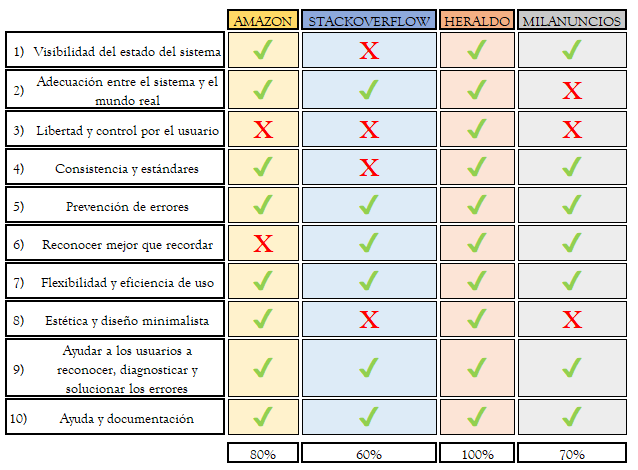
\includegraphics[scale = 0.80]{tabla_resumen.png}
\renewcommand{\figurename}{Tabla resumen}
\renewcommand{\thefigure}{}
\caption{\textit{10 principios heurísticos de usabilidad de Jakob Nielsen}}
\renewcommand{\figurename}{Fuente}
\caption{Propia}
\end{figure}
Gracias a está tabla resumen podemos decir de cada una de las páginas web:
\begin{itemize}
    \item \textbf{\underline{Amazon}} -- debería mejorar su \textbf{libertad y control por el usuario} (no se tan intrusivo a la hora de intentar vender su subscripción Prime) y también su \textbf{reconocer mejor que recordad} (por el mismo tema que en el apartado de libertad y control por el usuario).
    \item \textbf{\underline{StackOverflow}} -- debería mejorar varias cosas, como: su \textbf{visibilidad del estado del sistema} (aunque simplemente en su página inicial, ya que mezcla diferentes idiomas con diferentes temas, que no tienen porque ser lo que busques tu), su \textbf{libertad y control por el usuario} (por los errores que aparecen al añadir código en la página), su \textbf{consistencia y estándares}, (en ocasiones aparece y desaparece la barra lateral) y su \textbf{estética y diseño minimalista} (por la dificultad de a la hora de buscar la pregunta y las respuestas de los usuarios).
    \item \textbf{\underline{Heraldo}} -- no hay que modificar nada
    \item \textbf{\underline{Milanuncios}} -- había que modificar: \textbf{adecuación entre le sistema y el mundo real }("te hace ilusiones" permitiéndote acceder a ciertas partes de la página web en las que al final tienes que estar inscrito), \textbf{libertad y control por el usuario }(por la misma razón que la adecuación entre el sistema y el mundo real) y \textbf{estética y diseño minimalista} (ya que aparece algo sobrecargada la página web, al aparecer botones que solo deberías poder pulsar si ya estas logueado).
\end{itemize}
\end{document}
